\chapter{CƠ SỞ LÝ THUYẾT}
\section{Bảng và hình}
\subsection{Bảng}
Cách trình bày bảng~\ref{tab01} ... 

\begin{table}[!h]
\footnotesize
\caption{Bảng so sánh hiệu năng.}
\begin{tabular}{@{}l r r r@{}}
\hline
\multirow{1}{*}{Networks}	& Size (params.) & Speed (ms) & Acc. ($\%$)  \\ \hline
Method 1 &$	1.4\mathrm{M}	$&$	0.0390	$&$	87.66	$\\
Method 2	&$	6.1\mathrm{M}	$&$	0.0384	$&$	87.62	$\\
Method 3 &$	315\mathrm{K}	$&$	0.0586	$&$	89.91	$\\
MobileNetv2&$	2.2\mathrm{M}	$&$	0.0621	$&$	87.92	$\\
ResNet50&$	23.5\mathrm{M}	$&$	0.0683	$&$	87.34	$\\
Inception-V3&$	21.8\mathrm{M}	$&$	0.1059	$&$	89.94	$\\
EfficientNetb0&$	4.0\mathrm{M}	$&$	0.0823	$&$	89.47	$\\ 
Sim-RadComNet	&$	180\mathrm{K}		$&$	0.1055	$&$	87.46	$\\
Reg-RadComNet	&$	6.1\mathrm{M}		$&$	0.1270	$&$	89.47	$\\ \hline
RadComNet ($2$ RSA modules)	&$	102\mathrm{K}		$&$	0.0602	$&$	82.85	$\\
RadComNet ($3$ RSA modules)	&$	140\mathrm{K}		$&$	0.0644	$&$	86.85	$\\
RadComNet ($4$ RSA modules)	&$	178\mathrm{K}		$&$	0.0679	$&$	89.87	$\\
RadComNet ($5$ RSA modules)	&$	216\mathrm{K}		$&$	0.0712	$&$	90.56	$\\
RadComNet ($6$ RSA modules)	&$	254\mathrm{K}		$&$	0.0744	$&$	90.89	$\\
\hline
\end{tabular}
\label{tab01}
\end{table}

\begin{table}[!h]
\caption{Bảng điểm sinh viên}
\begin{tabular}{llll}
\hline
\multicolumn{1}{c}{MSSV} & \multicolumn{1}{c}{Họ} & \multicolumn{1}{c}{Tên} & \multicolumn{1}{c}{Điểm} \\ \hline
                         &                        & A                       & \multirow{2}{*}{8}       \\
                         &                        & B                       &                          \\
                         &                        &                         &                         
\end{tabular}
\label{tab02}
\end{table}

\subsection{Hình}
Hình được trình bày và tham khảo đến hình~\ref{fig01}...

\begin{figure}[!t]
	\centering
	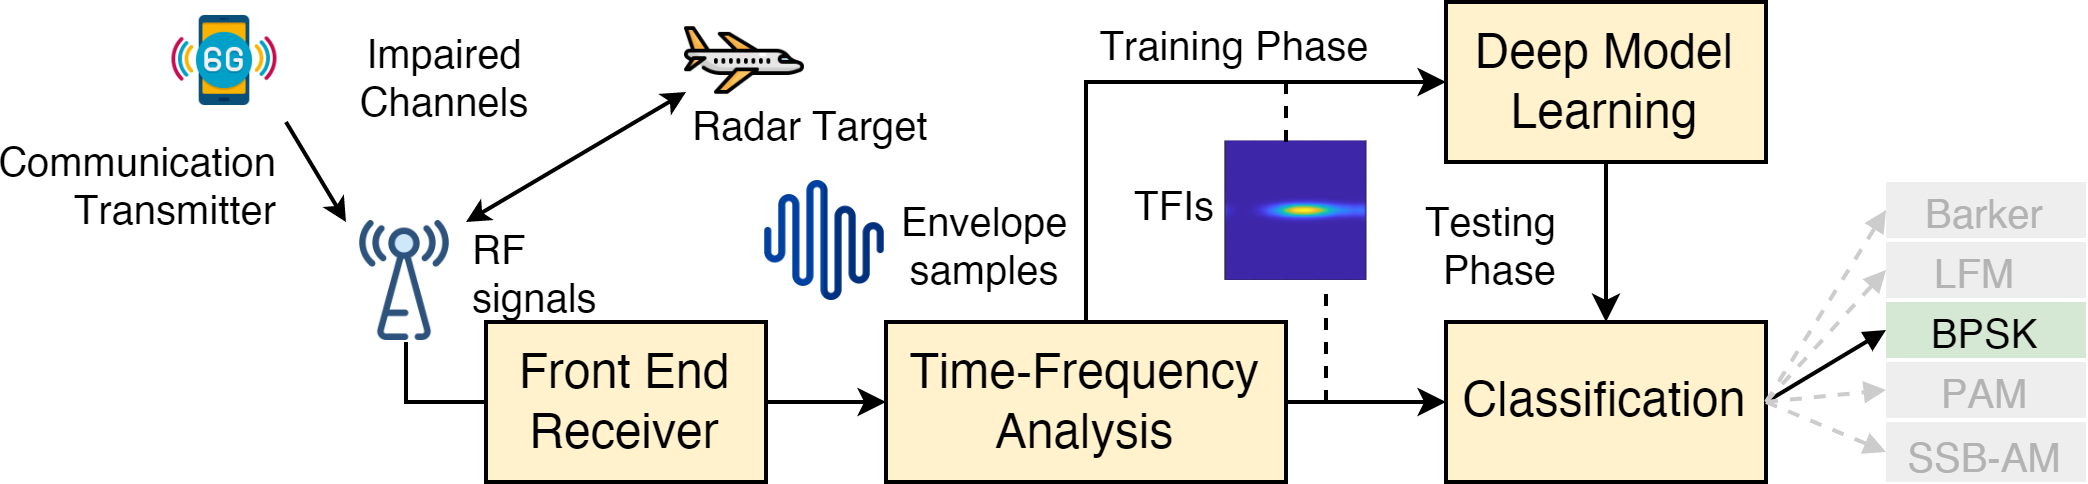
\includegraphics[width=14cm]{fig/fig01.png}    % hình được lưu trong thư mục fig (menu bên trái)
	\caption{Caption của hình là ...}
	\label{fig01}
\end{figure}

\subsubsection{Công thức toán học}
Công thức toán học được trình bày và đánh số tự động như trong công thức~(\ref{eqn01})...
\begin{equation}
h\left ( z \right )=\begin{cases}
z & \text{ if } z\geq 0 \\ 
0 & \text{ if } z < 0
\end{cases}.
\label{eqn01}
\end{equation}

\section{Cơ sở dữ liệu}
\subsection{Firebase Realtime Database}
Firebase Realtime Database ...
\subsubsection{Firebase A}
Firebase A là gì ...
\subsubsection{Firebase B}
Firebase B là gì ...
\subsection{Google Sheet}
Google Sheet là gì ...

